\documentclass[1p]{elsarticle_modified}
%\bibliographystyle{elsarticle-num}

%\usepackage[colorlinks]{hyperref}
%\usepackage{abbrmath_seonhwa} %\Abb, \Ascr, \Acal ,\Abf, \Afrak
\usepackage{amsfonts}
\usepackage{amssymb}
\usepackage{amsmath}
\usepackage{amsthm}
\usepackage{scalefnt}
\usepackage{amsbsy}
\usepackage{kotex}
\usepackage{caption}
\usepackage{subfig}
\usepackage{color}
\usepackage{graphicx}
\usepackage{xcolor} %% white, black, red, green, blue, cyan, magenta, yellow
\usepackage{float}
\usepackage{setspace}
\usepackage{hyperref}

\usepackage{tikz}
\usetikzlibrary{arrows}

\usepackage{multirow}
\usepackage{array} % fixed length table
\usepackage{hhline}

%%%%%%%%%%%%%%%%%%%%%
\makeatletter
\renewcommand*\env@matrix[1][\arraystretch]{%
	\edef\arraystretch{#1}%
	\hskip -\arraycolsep
	\let\@ifnextchar\new@ifnextchar
	\array{*\c@MaxMatrixCols c}}
\makeatother %https://tex.stackexchange.com/questions/14071/how-can-i-increase-the-line-spacing-in-a-matrix
%%%%%%%%%%%%%%%

\usepackage[normalem]{ulem}

\newcommand{\msout}[1]{\ifmmode\text{\sout{\ensuremath{#1}}}\else\sout{#1}\fi}
%SOURCE: \msout is \stkout macro in https://tex.stackexchange.com/questions/20609/strikeout-in-math-mode

\newcommand{\cancel}[1]{
	\ifmmode
	{\color{red}\msout{#1}}
	\else
	{\color{red}\sout{#1}}
	\fi
}

\newcommand{\add}[1]{
	{\color{blue}\uwave{#1}}
}

\newcommand{\replace}[2]{
	\ifmmode
	{\color{red}\msout{#1}}{\color{blue}\uwave{#2}}
	\else
	{\color{red}\sout{#1}}{\color{blue}\uwave{#2}}
	\fi
}

\newcommand{\Sol}{\mathcal{S}} %segment
\newcommand{\D}{D} %diagram
\newcommand{\A}{\mathcal{A}} %arc


%%%%%%%%%%%%%%%%%%%%%%%%%%%%%5 test

\def\sl{\operatorname{\textup{SL}}(2,\Cbb)}
\def\psl{\operatorname{\textup{PSL}}(2,\Cbb)}
\def\quan{\mkern 1mu \triangleright \mkern 1mu}

\theoremstyle{definition}
\newtheorem{thm}{Theorem}[section]
\newtheorem{prop}[thm]{Proposition}
\newtheorem{lem}[thm]{Lemma}
\newtheorem{ques}[thm]{Question}
\newtheorem{cor}[thm]{Corollary}
\newtheorem{defn}[thm]{Definition}
\newtheorem{exam}[thm]{Example}
\newtheorem{rmk}[thm]{Remark}
\newtheorem{alg}[thm]{Algorithm}

\newcommand{\I}{\sqrt{-1}}
\begin{document}

%\begin{frontmatter}
%
%\title{Boundary parabolic representations of knots up to 8 crossings}
%
%%% Group authors per affiliation:
%\author{Yunhi Cho} 
%\address{Department of Mathematics, University of Seoul, Seoul, Korea}
%\ead{yhcho@uos.ac.kr}
%
%
%\author{Seonhwa Kim} %\fnref{s_kim}}
%\address{Center for Geometry and Physics, Institute for Basic Science, Pohang, 37673, Korea}
%\ead{ryeona17@ibs.re.kr}
%
%\author{Hyuk Kim}
%\address{Department of Mathematical Sciences, Seoul National University, Seoul 08826, Korea}
%\ead{hyukkim@snu.ac.kr}
%
%\author{Seokbeom Yoon}
%\address{Department of Mathematical Sciences, Seoul National University, Seoul, 08826,  Korea}
%\ead{sbyoon15@snu.ac.kr}
%
%\begin{abstract}
%We find all boundary parabolic representation of knots up to 8 crossings.
%
%\end{abstract}
%\begin{keyword}
%    \MSC[2010] 57M25 
%\end{keyword}
%
%\end{frontmatter}

%\linenumbers
%\tableofcontents
%
\newcommand\colored[1]{\textcolor{white}{\rule[-0.35ex]{0.8em}{1.4ex}}\kern-0.8em\color{red} #1}%
%\newcommand\colored[1]{\textcolor{white}{ #1}\kern-2.17ex	\textcolor{white}{ #1}\kern-1.81ex	\textcolor{white}{ #1}\kern-2.15ex\color{red}#1	}

{\Large $\underline{11a_{164}~(K11a_{164})}$}

\setlength{\tabcolsep}{10pt}
\renewcommand{\arraystretch}{1.6}
\vspace{1cm}\begin{tabular}{m{100pt}>{\centering\arraybackslash}m{274pt}}
\multirow{5}{120pt}{
	\centering
	\includegraphics[width=112pt]{../../../GIT/diagram.site/Diagrams/png/413_11a_164.png}\\
\ \ \ A knot diagram\footnotemark}&
\allowdisplaybreaks
\textbf{Linearized knot diagam} \\
\cline{2-2}
 &
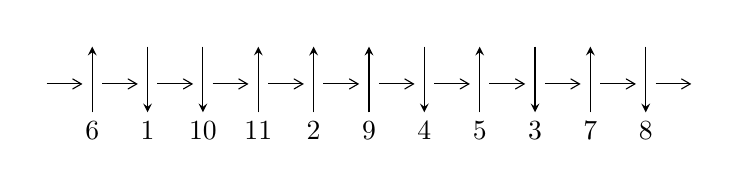
\begin{tikzpicture}[x=20pt, y=17pt]
	% nodes
	\node (C0) at (0, 0) {};
	\node (C1) at (1, 0) {};
	\node (C1U) at (1, +1) {};
	\node (C1D) at (1, -1) {6};

	\node (C2) at (2, 0) {};
	\node (C2U) at (2, +1) {};
	\node (C2D) at (2, -1) {1};

	\node (C3) at (3, 0) {};
	\node (C3U) at (3, +1) {};
	\node (C3D) at (3, -1) {10};

	\node (C4) at (4, 0) {};
	\node (C4U) at (4, +1) {};
	\node (C4D) at (4, -1) {11};

	\node (C5) at (5, 0) {};
	\node (C5U) at (5, +1) {};
	\node (C5D) at (5, -1) {2};

	\node (C6) at (6, 0) {};
	\node (C6U) at (6, +1) {};
	\node (C6D) at (6, -1) {9};

	\node (C7) at (7, 0) {};
	\node (C7U) at (7, +1) {};
	\node (C7D) at (7, -1) {4};

	\node (C8) at (8, 0) {};
	\node (C8U) at (8, +1) {};
	\node (C8D) at (8, -1) {5};

	\node (C9) at (9, 0) {};
	\node (C9U) at (9, +1) {};
	\node (C9D) at (9, -1) {3};

	\node (C10) at (10, 0) {};
	\node (C10U) at (10, +1) {};
	\node (C10D) at (10, -1) {7};

	\node (C11) at (11, 0) {};
	\node (C11U) at (11, +1) {};
	\node (C11D) at (11, -1) {8};
	\node (C12) at (12, 0) {};

	% arrows
	\draw[->,>={angle 60}]
	(C0) edge (C1) (C1) edge (C2) (C2) edge (C3) (C3) edge (C4) (C4) edge (C5) (C5) edge (C6) (C6) edge (C7) (C7) edge (C8) (C8) edge (C9) (C9) edge (C10) (C10) edge (C11) (C11) edge (C12) ;	\draw[->,>=stealth]
	(C1D) edge (C1U) (C2U) edge (C2D) (C3U) edge (C3D) (C4D) edge (C4U) (C5D) edge (C5U) (C6D) edge (C6U) (C7U) edge (C7D) (C8D) edge (C8U) (C9U) edge (C9D) (C10D) edge (C10U) (C11U) edge (C11D) ;
	\end{tikzpicture} \\
\hhline{~~} \\& 
\textbf{Solving Sequence} \\ \cline{2-2} 
 &
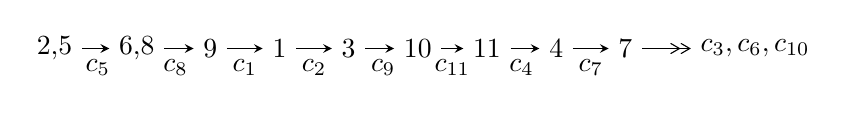
\begin{tikzpicture}[x=25pt, y=7pt]
	% node
	\node (A0) at (-1/8, 0) {2,5};
	\node (A1) at (17/16, 0) {6,8};
	\node (A2) at (17/8, 0) {9};
	\node (A3) at (25/8, 0) {1};
	\node (A4) at (33/8, 0) {3};
	\node (A5) at (41/8, 0) {10};
	\node (A6) at (49/8, 0) {11};
	\node (A7) at (57/8, 0) {4};
	\node (A8) at (65/8, 0) {7};
	\node (C1) at (1/2, -1) {$c_{5}$};
	\node (C2) at (13/8, -1) {$c_{8}$};
	\node (C3) at (21/8, -1) {$c_{1}$};
	\node (C4) at (29/8, -1) {$c_{2}$};
	\node (C5) at (37/8, -1) {$c_{9}$};
	\node (C6) at (45/8, -1) {$c_{11}$};
	\node (C7) at (53/8, -1) {$c_{4}$};
	\node (C8) at (61/8, -1) {$c_{7}$};
	\node (A9) at (10, 0) {$c_{3},c_{6},c_{10}$};

	% edge
	\draw[->,>=stealth]	
	(A0) edge (A1) (A1) edge (A2) (A2) edge (A3) (A3) edge (A4) (A4) edge (A5) (A5) edge (A6) (A6) edge (A7) (A7) edge (A8) ;
	\draw[->>,>={angle 60}]	
	(A8) edge (A9);
\end{tikzpicture} \\ 

\end{tabular} \\

\footnotetext{
The image of knot diagram is generated by the software ``\textbf{Draw programme}" developed by Andrew Bartholomew(\url{http://www.layer8.co.uk/maths/draw/index.htm\#Running-draw}), where we modified some parts for our purpose(\url{https://github.com/CATsTAILs/LinksPainter}).
}\phantom \\ \newline 
\centering \textbf{Ideals for irreducible components\footnotemark of $X_{\text{par}}$} 
 
\begin{align*}
I^u_{1}&=\langle 
-9.08044\times10^{141} u^{100}-1.16506\times10^{142} u^{99}+\cdots+2.96438\times10^{142} b+6.72571\times10^{142},\\
\phantom{I^u_{1}}&\phantom{= \langle  }-1.52478\times10^{143} u^{100}+2.53452\times10^{142} u^{99}+\cdots+2.96438\times10^{142} a+2.83966\times10^{143},\\
\phantom{I^u_{1}}&\phantom{= \langle  }u^{101}+24 u^{99}+\cdots+10 u+1\rangle \\
I^u_{2}&=\langle 
- u^{16}- u^{15}-5 u^{14}-4 u^{13}-10 u^{12}-6 u^{11}-11 u^{10}-4 u^9-6 u^8+u^7-3 u^6+2 u^5-3 u^4+u^3+b+1,\\
\phantom{I^u_{2}}&\phantom{= \langle  }-4 u^{16}-10 u^{15}+\cdots+a+6,\;u^{17}+u^{16}+\cdots+2 u-1\rangle \\
\\
\end{align*}
\raggedright * 2 irreducible components of $\dim_{\mathbb{C}}=0$, with total 118 representations.\\
\footnotetext{All coefficients of polynomials are rational numbers. But the coefficients are sometimes approximated in decimal forms when there is not enough margin.}
\newpage
\renewcommand{\arraystretch}{1}
\centering \section*{I. $I^u_{1}= \langle -9.08\times10^{141} u^{100}-1.17\times10^{142} u^{99}+\cdots+2.96\times10^{142} b+6.73\times10^{142},\;-1.52\times10^{143} u^{100}+2.53\times10^{142} u^{99}+\cdots+2.96\times10^{142} a+2.84\times10^{143},\;u^{101}+24 u^{99}+\cdots+10 u+1 \rangle$}
\flushleft \textbf{(i) Arc colorings}\\
\begin{tabular}{m{7pt} m{180pt} m{7pt} m{180pt} }
\flushright $a_{2}=$&$\begin{pmatrix}0\\u\end{pmatrix}$ \\
\flushright $a_{5}=$&$\begin{pmatrix}1\\0\end{pmatrix}$ \\
\flushright $a_{6}=$&$\begin{pmatrix}1\\- u^2\end{pmatrix}$ \\
\flushright $a_{8}=$&$\begin{pmatrix}5.14368 u^{100}-0.854991 u^{99}+\cdots-75.8410 u-9.57926\\0.306318 u^{100}+0.393021 u^{99}+\cdots-11.1105 u-2.26884\end{pmatrix}$ \\
\flushright $a_{9}=$&$\begin{pmatrix}5.45000 u^{100}-0.461970 u^{99}+\cdots-86.9515 u-11.8481\\0.306318 u^{100}+0.393021 u^{99}+\cdots-11.1105 u-2.26884\end{pmatrix}$ \\
\flushright $a_{1}=$&$\begin{pmatrix}- u\\u^3+u\end{pmatrix}$ \\
\flushright $a_{3}=$&$\begin{pmatrix}- u^3\\u^5+u^3+u\end{pmatrix}$ \\
\flushright $a_{10}=$&$\begin{pmatrix}5.21197 u^{100}-2.09654 u^{99}+\cdots-105.903 u-13.5218\\-0.375750 u^{100}+0.0665634 u^{99}+\cdots-5.48782 u-1.77008\end{pmatrix}$ \\
\flushright $a_{11}=$&$\begin{pmatrix}1.79088 u^{100}-2.36678 u^{99}+\cdots-67.2269 u-7.13448\\-1.52592 u^{100}-1.16036 u^{99}+\cdots-19.1077 u-2.00447\end{pmatrix}$ \\
\flushright $a_{4}=$&$\begin{pmatrix}-1.60316 u^{100}+4.26183 u^{99}+\cdots+81.9912 u+8.94626\\-0.148855 u^{100}-2.54143 u^{99}+\cdots-9.70613 u-0.621772\end{pmatrix}$ \\
\flushright $a_{7}=$&$\begin{pmatrix}-1.79064 u^{100}+3.85132 u^{99}+\cdots+96.9928 u+5.13132\\0.204887 u^{100}+0.0480139 u^{99}+\cdots+2.60472 u-1.56299\end{pmatrix}$\\ \flushright $a_{7}=$&$\begin{pmatrix}-1.79064 u^{100}+3.85132 u^{99}+\cdots+96.9928 u+5.13132\\0.204887 u^{100}+0.0480139 u^{99}+\cdots+2.60472 u-1.56299\end{pmatrix}$\\&\end{tabular}
\flushleft \textbf{(ii) Obstruction class $= -1$}\\~\\
\flushleft \textbf{(iii) Cusp Shapes $= -75.9603 u^{100}+17.6410 u^{99}+\cdots+792.020 u+79.1726$}\\~\\
\newpage\renewcommand{\arraystretch}{1}
\flushleft \textbf{(iv) u-Polynomials at the component}\newline \\
\begin{tabular}{m{50pt}|m{274pt}}
Crossings & \hspace{64pt}u-Polynomials at each crossing \\
\hline $$\begin{aligned}c_{1},c_{5}\end{aligned}$$&$\begin{aligned}
&u^{101}+24 u^{99}+\cdots+10 u+1
\end{aligned}$\\
\hline $$\begin{aligned}c_{2}\end{aligned}$$&$\begin{aligned}
&u^{101}+48 u^{100}+\cdots+56 u-1
\end{aligned}$\\
\hline $$\begin{aligned}c_{3},c_{9}\end{aligned}$$&$\begin{aligned}
&u^{101}+2 u^{100}+\cdots+2225 u+419
\end{aligned}$\\
\hline $$\begin{aligned}c_{4}\end{aligned}$$&$\begin{aligned}
&u^{101}- u^{100}+\cdots+27 u-1
\end{aligned}$\\
\hline $$\begin{aligned}c_{6}\end{aligned}$$&$\begin{aligned}
&u^{101}-2 u^{100}+\cdots+509 u-103
\end{aligned}$\\
\hline $$\begin{aligned}c_{7}\end{aligned}$$&$\begin{aligned}
&u^{101}+3 u^{100}+\cdots+2286 u-617
\end{aligned}$\\
\hline $$\begin{aligned}c_{8}\end{aligned}$$&$\begin{aligned}
&u^{101}+2 u^{100}+\cdots-3009 u-289
\end{aligned}$\\
\hline $$\begin{aligned}c_{10}\end{aligned}$$&$\begin{aligned}
&u^{101}+u^{100}+\cdots+18 u+1
\end{aligned}$\\
\hline $$\begin{aligned}c_{11}\end{aligned}$$&$\begin{aligned}
&u^{101}+3 u^{100}+\cdots-550 u-25
\end{aligned}$\\
\hline
\end{tabular}\\~\\
\newpage\renewcommand{\arraystretch}{1}
\flushleft \textbf{(v) Riley Polynomials at the component}\newline \\
\begin{tabular}{m{50pt}|m{274pt}}
Crossings & \hspace{64pt}Riley Polynomials at each crossing \\
\hline $$\begin{aligned}c_{1},c_{5}\end{aligned}$$&$\begin{aligned}
&y^{101}+48 y^{100}+\cdots+56 y-1
\end{aligned}$\\
\hline $$\begin{aligned}c_{2}\end{aligned}$$&$\begin{aligned}
&y^{101}+16 y^{100}+\cdots+5112 y-1
\end{aligned}$\\
\hline $$\begin{aligned}c_{3},c_{9}\end{aligned}$$&$\begin{aligned}
&y^{101}-66 y^{100}+\cdots+4179665 y-175561
\end{aligned}$\\
\hline $$\begin{aligned}c_{4}\end{aligned}$$&$\begin{aligned}
&y^{101}-3 y^{100}+\cdots+397 y-1
\end{aligned}$\\
\hline $$\begin{aligned}c_{6}\end{aligned}$$&$\begin{aligned}
&y^{101}+2 y^{100}+\cdots+495157 y-10609
\end{aligned}$\\
\hline $$\begin{aligned}c_{7}\end{aligned}$$&$\begin{aligned}
&y^{101}-23 y^{100}+\cdots+17244956 y-380689
\end{aligned}$\\
\hline $$\begin{aligned}c_{8}\end{aligned}$$&$\begin{aligned}
&y^{101}-10 y^{100}+\cdots+435523 y-83521
\end{aligned}$\\
\hline $$\begin{aligned}c_{10}\end{aligned}$$&$\begin{aligned}
&y^{101}+15 y^{100}+\cdots+48 y-1
\end{aligned}$\\
\hline $$\begin{aligned}c_{11}\end{aligned}$$&$\begin{aligned}
&y^{101}-5 y^{100}+\cdots+430150 y-625
\end{aligned}$\\
\hline
\end{tabular}\\~\\
\newpage\flushleft \textbf{(vi) Complex Volumes and Cusp Shapes}
$$\begin{array}{c|c|c}  
\text{Solutions to }I^u_{1}& \I (\text{vol} + \sqrt{-1}CS) & \text{Cusp shape}\\
 \hline 
\begin{aligned}
u &= \phantom{-}0.799338 + 0.603896 I \\
a &= \phantom{-}1.310790 + 0.397626 I \\
b &= -0.730027 + 0.237935 I\end{aligned}
 & \phantom{-}0.67147 - 3.20721 I & \phantom{-0.000000 } 0 \\ \hline\begin{aligned}
u &= \phantom{-}0.799338 - 0.603896 I \\
a &= \phantom{-}1.310790 - 0.397626 I \\
b &= -0.730027 - 0.237935 I\end{aligned}
 & \phantom{-}0.67147 + 3.20721 I & \phantom{-0.000000 } 0 \\ \hline\begin{aligned}
u &= \phantom{-}0.920784 + 0.379494 I \\
a &= -1.36311 + 0.74527 I \\
b &= \phantom{-}1.27183 - 0.84399 I\end{aligned}
 & -0.83041 - 12.65940 I & \phantom{-0.000000 } 0 \\ \hline\begin{aligned}
u &= \phantom{-}0.920784 - 0.379494 I \\
a &= -1.36311 - 0.74527 I \\
b &= \phantom{-}1.27183 + 0.84399 I\end{aligned}
 & -0.83041 + 12.65940 I & \phantom{-0.000000 } 0 \\ \hline\begin{aligned}
u &= \phantom{-}0.310097 + 0.962923 I \\
a &= \phantom{-}0.873648 + 0.529676 I \\
b &= \phantom{-}0.683779 - 1.049460 I\end{aligned}
 & -0.399141 + 1.242870 I & \phantom{-0.000000 } 0 \\ \hline\begin{aligned}
u &= \phantom{-}0.310097 - 0.962923 I \\
a &= \phantom{-}0.873648 - 0.529676 I \\
b &= \phantom{-}0.683779 + 1.049460 I\end{aligned}
 & -0.399141 - 1.242870 I & \phantom{-0.000000 } 0 \\ \hline\begin{aligned}
u &= -0.914060 + 0.352085 I \\
a &= -0.588282 - 0.618097 I \\
b &= \phantom{-}0.767034 + 0.712223 I\end{aligned}
 & -2.33944 + 4.55777 I & \phantom{-0.000000 } 0 \\ \hline\begin{aligned}
u &= -0.914060 - 0.352085 I \\
a &= -0.588282 + 0.618097 I \\
b &= \phantom{-}0.767034 - 0.712223 I\end{aligned}
 & -2.33944 - 4.55777 I & \phantom{-0.000000 } 0 \\ \hline\begin{aligned}
u &= \phantom{-}0.834355 + 0.503525 I \\
a &= -0.668685 - 0.367928 I \\
b &= \phantom{-}0.780605 + 0.089667 I\end{aligned}
 & \phantom{-}3.71124 + 3.14543 I & \phantom{-0.000000 } 0 \\ \hline\begin{aligned}
u &= \phantom{-}0.834355 - 0.503525 I \\
a &= -0.668685 + 0.367928 I \\
b &= \phantom{-}0.780605 - 0.089667 I\end{aligned}
 & \phantom{-}3.71124 - 3.14543 I & \phantom{-0.000000 } 0\\
 \hline 
 \end{array}$$\newpage$$\begin{array}{c|c|c}  
\text{Solutions to }I^u_{1}& \I (\text{vol} + \sqrt{-1}CS) & \text{Cusp shape}\\
 \hline 
\begin{aligned}
u &= \phantom{-}0.414857 + 0.874591 I \\
a &= -2.48341 - 0.53136 I \\
b &= \phantom{-}0.11393 + 2.94906 I\end{aligned}
 & -1.97371 + 1.74177 I & \phantom{-0.000000 } 0 \\ \hline\begin{aligned}
u &= \phantom{-}0.414857 - 0.874591 I \\
a &= -2.48341 + 0.53136 I \\
b &= \phantom{-}0.11393 - 2.94906 I\end{aligned}
 & -1.97371 - 1.74177 I & \phantom{-0.000000 } 0 \\ \hline\begin{aligned}
u &= -0.156554 + 0.939549 I \\
a &= \phantom{-}0.107048 + 0.818381 I \\
b &= \phantom{-}0.443879 + 1.017760 I\end{aligned}
 & -3.36242 + 1.21904 I & \phantom{-0.000000 } 0 \\ \hline\begin{aligned}
u &= -0.156554 - 0.939549 I \\
a &= \phantom{-}0.107048 - 0.818381 I \\
b &= \phantom{-}0.443879 - 1.017760 I\end{aligned}
 & -3.36242 - 1.21904 I & \phantom{-0.000000 } 0 \\ \hline\begin{aligned}
u &= -0.812488 + 0.488151 I \\
a &= -1.29297 - 1.09727 I \\
b &= \phantom{-}1.30092 + 0.77115 I\end{aligned}
 & \phantom{-}3.68064 + 6.67564 I & \phantom{-0.000000 } 0 \\ \hline\begin{aligned}
u &= -0.812488 - 0.488151 I \\
a &= -1.29297 + 1.09727 I \\
b &= \phantom{-}1.30092 - 0.77115 I\end{aligned}
 & \phantom{-}3.68064 - 6.67564 I & \phantom{-0.000000 } 0 \\ \hline\begin{aligned}
u &= \phantom{-}0.472749 + 0.956015 I \\
a &= \phantom{-}1.29828 - 0.99813 I \\
b &= -1.72376 + 0.36555 I\end{aligned}
 & -2.59160 + 2.64890 I & \phantom{-0.000000 } 0 \\ \hline\begin{aligned}
u &= \phantom{-}0.472749 - 0.956015 I \\
a &= \phantom{-}1.29828 + 0.99813 I \\
b &= -1.72376 - 0.36555 I\end{aligned}
 & -2.59160 - 2.64890 I & \phantom{-0.000000 } 0 \\ \hline\begin{aligned}
u &= -0.711647 + 0.603130 I \\
a &= \phantom{-}1.27586 + 0.82927 I \\
b &= -0.713650 - 0.372777 I\end{aligned}
 & \phantom{-}0.97787 + 2.04675 I & \phantom{-0.000000 } 0 \\ \hline\begin{aligned}
u &= -0.711647 - 0.603130 I \\
a &= \phantom{-}1.27586 - 0.82927 I \\
b &= -0.713650 + 0.372777 I\end{aligned}
 & \phantom{-}0.97787 - 2.04675 I & \phantom{-0.000000 } 0\\
 \hline 
 \end{array}$$\newpage$$\begin{array}{c|c|c}  
\text{Solutions to }I^u_{1}& \I (\text{vol} + \sqrt{-1}CS) & \text{Cusp shape}\\
 \hline 
\begin{aligned}
u &= -0.619610 + 0.688764 I \\
a &= \phantom{-}1.303250 - 0.202527 I \\
b &= -0.978922 - 0.237953 I\end{aligned}
 & \phantom{-}3.95086 - 0.15387 I & \phantom{-0.000000 } 0 \\ \hline\begin{aligned}
u &= -0.619610 - 0.688764 I \\
a &= \phantom{-}1.303250 + 0.202527 I \\
b &= -0.978922 + 0.237953 I\end{aligned}
 & \phantom{-}3.95086 + 0.15387 I & \phantom{-0.000000 } 0 \\ \hline\begin{aligned}
u &= \phantom{-}0.614599 + 0.687148 I \\
a &= -0.278610 + 0.955094 I \\
b &= \phantom{-}0.780571 - 0.602224 I\end{aligned}
 & \phantom{-}0.44573 + 1.61901 I & \phantom{-0.000000 } 0 \\ \hline\begin{aligned}
u &= \phantom{-}0.614599 - 0.687148 I \\
a &= -0.278610 - 0.955094 I \\
b &= \phantom{-}0.780571 + 0.602224 I\end{aligned}
 & \phantom{-}0.44573 - 1.61901 I & \phantom{-0.000000 } 0 \\ \hline\begin{aligned}
u &= -0.159716 + 1.068970 I \\
a &= \phantom{-}0.779544 + 0.696041 I \\
b &= \phantom{-}0.648363 + 0.903082 I\end{aligned}
 & -3.30571 + 2.25191 I & \phantom{-0.000000 } 0 \\ \hline\begin{aligned}
u &= -0.159716 - 1.068970 I \\
a &= \phantom{-}0.779544 - 0.696041 I \\
b &= \phantom{-}0.648363 - 0.903082 I\end{aligned}
 & -3.30571 - 2.25191 I & \phantom{-0.000000 } 0 \\ \hline\begin{aligned}
u &= \phantom{-}0.446085 + 0.987433 I \\
a &= -2.74444 + 0.81201 I \\
b &= \phantom{-}0.603591 + 0.661833 I\end{aligned}
 & -4.95602 + 7.28899 I & \phantom{-0.000000 } 0 \\ \hline\begin{aligned}
u &= \phantom{-}0.446085 - 0.987433 I \\
a &= -2.74444 - 0.81201 I \\
b &= \phantom{-}0.603591 - 0.661833 I\end{aligned}
 & -4.95602 - 7.28899 I & \phantom{-0.000000 } 0 \\ \hline\begin{aligned}
u &= \phantom{-}1.006780 + 0.413097 I \\
a &= \phantom{-}1.183050 - 0.359917 I \\
b &= -0.953599 + 0.459118 I\end{aligned}
 & -1.20543 - 2.91368 I & \phantom{-0.000000 } 0 \\ \hline\begin{aligned}
u &= \phantom{-}1.006780 - 0.413097 I \\
a &= \phantom{-}1.183050 + 0.359917 I \\
b &= -0.953599 - 0.459118 I\end{aligned}
 & -1.20543 + 2.91368 I & \phantom{-0.000000 } 0\\
 \hline 
 \end{array}$$\newpage$$\begin{array}{c|c|c}  
\text{Solutions to }I^u_{1}& \I (\text{vol} + \sqrt{-1}CS) & \text{Cusp shape}\\
 \hline 
\begin{aligned}
u &= -0.356062 + 1.034300 I \\
a &= \phantom{-}1.90863 + 0.96870 I \\
b &= -1.04466 + 1.05860 I\end{aligned}
 & -6.47568 + 2.60950 I & \phantom{-0.000000 } 0 \\ \hline\begin{aligned}
u &= -0.356062 - 1.034300 I \\
a &= \phantom{-}1.90863 - 0.96870 I \\
b &= -1.04466 - 1.05860 I\end{aligned}
 & -6.47568 - 2.60950 I & \phantom{-0.000000 } 0 \\ \hline\begin{aligned}
u &= \phantom{-}0.463350 + 1.009350 I \\
a &= \phantom{-}0.547639 - 0.776583 I \\
b &= \phantom{-}0.466122 - 1.198110 I\end{aligned}
 & -4.78444 - 1.35131 I & \phantom{-0.000000 } 0 \\ \hline\begin{aligned}
u &= \phantom{-}0.463350 - 1.009350 I \\
a &= \phantom{-}0.547639 + 0.776583 I \\
b &= \phantom{-}0.466122 + 1.198110 I\end{aligned}
 & -4.78444 + 1.35131 I & \phantom{-0.000000 } 0 \\ \hline\begin{aligned}
u &= -0.593448 + 0.943581 I \\
a &= -0.96895 - 1.43132 I \\
b &= \phantom{-}0.731080 - 0.425982 I\end{aligned}
 & \phantom{-}3.17647 - 4.63483 I & \phantom{-0.000000 } 0 \\ \hline\begin{aligned}
u &= -0.593448 - 0.943581 I \\
a &= -0.96895 + 1.43132 I \\
b &= \phantom{-}0.731080 + 0.425982 I\end{aligned}
 & \phantom{-}3.17647 + 4.63483 I & \phantom{-0.000000 } 0 \\ \hline\begin{aligned}
u &= \phantom{-}0.026019 + 1.128800 I \\
a &= -0.417275 - 0.110011 I \\
b &= -0.594637 - 0.897589 I\end{aligned}
 & -2.11387 + 5.01998 I & \phantom{-0.000000 } 0 \\ \hline\begin{aligned}
u &= \phantom{-}0.026019 - 1.128800 I \\
a &= -0.417275 + 0.110011 I \\
b &= -0.594637 + 0.897589 I\end{aligned}
 & -2.11387 - 5.01998 I & \phantom{-0.000000 } 0 \\ \hline\begin{aligned}
u &= \phantom{-}0.571043 + 0.979201 I \\
a &= \phantom{-}1.75185 - 0.23420 I \\
b &= -0.92445 - 1.33397 I\end{aligned}
 & -0.50863 + 3.05407 I & \phantom{-0.000000 } 0 \\ \hline\begin{aligned}
u &= \phantom{-}0.571043 - 0.979201 I \\
a &= \phantom{-}1.75185 + 0.23420 I \\
b &= -0.92445 + 1.33397 I\end{aligned}
 & -0.50863 - 3.05407 I & \phantom{-0.000000 } 0\\
 \hline 
 \end{array}$$\newpage$$\begin{array}{c|c|c}  
\text{Solutions to }I^u_{1}& \I (\text{vol} + \sqrt{-1}CS) & \text{Cusp shape}\\
 \hline 
\begin{aligned}
u &= -0.851203 + 0.755593 I \\
a &= -1.107360 + 0.060680 I \\
b &= \phantom{-}0.969445 - 0.244990 I\end{aligned}
 & \phantom{-}1.46871 - 8.32039 I & \phantom{-0.000000 } 0 \\ \hline\begin{aligned}
u &= -0.851203 - 0.755593 I \\
a &= -1.107360 - 0.060680 I \\
b &= \phantom{-}0.969445 + 0.244990 I\end{aligned}
 & \phantom{-}1.46871 + 8.32039 I & \phantom{-0.000000 } 0 \\ \hline\begin{aligned}
u &= -0.751900 + 0.416167 I \\
a &= \phantom{-}1.25275 + 0.66263 I \\
b &= -1.11700 - 0.97222 I\end{aligned}
 & \phantom{-}1.45805 + 4.32698 I & \phantom{-0.000000 } 0 \\ \hline\begin{aligned}
u &= -0.751900 - 0.416167 I \\
a &= \phantom{-}1.25275 - 0.66263 I \\
b &= -1.11700 + 0.97222 I\end{aligned}
 & \phantom{-}1.45805 - 4.32698 I & \phantom{-0.000000 } 0 \\ \hline\begin{aligned}
u &= \phantom{-}0.686788 + 0.515849 I \\
a &= \phantom{-}1.360940 + 0.111989 I \\
b &= -1.084070 - 0.393308 I\end{aligned}
 & \phantom{-}2.01265 + 1.89682 I & \phantom{-0.000000 } 0 \\ \hline\begin{aligned}
u &= \phantom{-}0.686788 - 0.515849 I \\
a &= \phantom{-}1.360940 - 0.111989 I \\
b &= -1.084070 + 0.393308 I\end{aligned}
 & \phantom{-}2.01265 - 1.89682 I & \phantom{-0.000000 } 0 \\ \hline\begin{aligned}
u &= -0.329654 + 1.104690 I \\
a &= -0.961036 - 0.873809 I \\
b &= \phantom{-}0.973345 - 0.089544 I\end{aligned}
 & -6.08185 - 3.72513 I & \phantom{-0.000000 } 0 \\ \hline\begin{aligned}
u &= -0.329654 - 1.104690 I \\
a &= -0.961036 + 0.873809 I \\
b &= \phantom{-}0.973345 + 0.089544 I\end{aligned}
 & -6.08185 + 3.72513 I & \phantom{-0.000000 } 0 \\ \hline\begin{aligned}
u &= \phantom{-}0.402510 + 0.742669 I \\
a &= -1.32349 + 2.16488 I \\
b &= \phantom{-}1.223860 + 0.498277 I\end{aligned}
 & -1.82096 + 1.07594 I & \phantom{-0.000000 } 0 \\ \hline\begin{aligned}
u &= \phantom{-}0.402510 - 0.742669 I \\
a &= -1.32349 - 2.16488 I \\
b &= \phantom{-}1.223860 - 0.498277 I\end{aligned}
 & -1.82096 - 1.07594 I & \phantom{-0.000000 } 0\\
 \hline 
 \end{array}$$\newpage$$\begin{array}{c|c|c}  
\text{Solutions to }I^u_{1}& \I (\text{vol} + \sqrt{-1}CS) & \text{Cusp shape}\\
 \hline 
\begin{aligned}
u &= -0.498083 + 1.052540 I \\
a &= -0.869818 + 0.501520 I \\
b &= -0.64201 - 1.73281 I\end{aligned}
 & -5.52278 - 9.23097 I & \phantom{-0.000000 } 0 \\ \hline\begin{aligned}
u &= -0.498083 - 1.052540 I \\
a &= -0.869818 - 0.501520 I \\
b &= -0.64201 + 1.73281 I\end{aligned}
 & -5.52278 + 9.23097 I & \phantom{-0.000000 } 0 \\ \hline\begin{aligned}
u &= -0.803342 + 0.843458 I \\
a &= \phantom{-}0.853853 + 0.788546 I \\
b &= -0.772508 - 0.059619 I\end{aligned}
 & \phantom{-}1.15621 + 2.31115 I & \phantom{-0.000000 } 0 \\ \hline\begin{aligned}
u &= -0.803342 - 0.843458 I \\
a &= \phantom{-}0.853853 - 0.788546 I \\
b &= -0.772508 + 0.059619 I\end{aligned}
 & \phantom{-}1.15621 - 2.31115 I & \phantom{-0.000000 } 0 \\ \hline\begin{aligned}
u &= -0.453521 + 1.073760 I \\
a &= -0.205523 + 0.115628 I \\
b &= \phantom{-}0.339218 + 0.818234 I\end{aligned}
 & -5.48767 - 3.61474 I & \phantom{-0.000000 } 0 \\ \hline\begin{aligned}
u &= -0.453521 - 1.073760 I \\
a &= -0.205523 - 0.115628 I \\
b &= \phantom{-}0.339218 - 0.818234 I\end{aligned}
 & -5.48767 + 3.61474 I & \phantom{-0.000000 } 0 \\ \hline\begin{aligned}
u &= -0.424837 + 1.089140 I \\
a &= -0.953607 + 0.007477 I \\
b &= \phantom{-}0.254632 + 0.237622 I\end{aligned}
 & -5.68517 - 3.63758 I & \phantom{-0.000000 } 0 \\ \hline\begin{aligned}
u &= -0.424837 - 1.089140 I \\
a &= -0.953607 - 0.007477 I \\
b &= \phantom{-}0.254632 - 0.237622 I\end{aligned}
 & -5.68517 + 3.63758 I & \phantom{-0.000000 } 0 \\ \hline\begin{aligned}
u &= -0.829751\phantom{ +0.000000I} \\
a &= \phantom{-}1.76369\phantom{ +0.000000I} \\
b &= -0.808831\phantom{ +0.000000I}\end{aligned}
 & -2.37595\phantom{ +0.000000I} & -7.91280\phantom{ +0.000000I} \\ \hline\begin{aligned}
u &= \phantom{-}0.308021 + 0.765503 I \\
a &= \phantom{-}1.85520 - 2.58678 I \\
b &= -0.180074 + 0.323037 I\end{aligned}
 & -3.96508 - 3.96334 I & \phantom{-0.000000 } 0\\
 \hline 
 \end{array}$$\newpage$$\begin{array}{c|c|c}  
\text{Solutions to }I^u_{1}& \I (\text{vol} + \sqrt{-1}CS) & \text{Cusp shape}\\
 \hline 
\begin{aligned}
u &= \phantom{-}0.308021 - 0.765503 I \\
a &= \phantom{-}1.85520 + 2.58678 I \\
b &= -0.180074 - 0.323037 I\end{aligned}
 & -3.96508 + 3.96334 I & \phantom{-0.000000 } 0 \\ \hline\begin{aligned}
u &= \phantom{-}0.543567 + 1.047650 I \\
a &= -1.63400 + 1.40042 I \\
b &= \phantom{-}1.63666 + 0.90355 I\end{aligned}
 & \phantom{-}1.25180 + 5.00759 I & \phantom{-0.000000 } 0 \\ \hline\begin{aligned}
u &= \phantom{-}0.543567 - 1.047650 I \\
a &= -1.63400 - 1.40042 I \\
b &= \phantom{-}1.63666 - 0.90355 I\end{aligned}
 & \phantom{-}1.25180 - 5.00759 I & \phantom{-0.000000 } 0 \\ \hline\begin{aligned}
u &= \phantom{-}0.565766 + 1.046080 I \\
a &= -0.531297 + 1.005030 I \\
b &= \phantom{-}1.011750 - 0.024388 I\end{aligned}
 & \phantom{-}0.43832 + 2.94973 I & \phantom{-0.000000 } 0 \\ \hline\begin{aligned}
u &= \phantom{-}0.565766 - 1.046080 I \\
a &= -0.531297 - 1.005030 I \\
b &= \phantom{-}1.011750 + 0.024388 I\end{aligned}
 & \phantom{-}0.43832 - 2.94973 I & \phantom{-0.000000 } 0 \\ \hline\begin{aligned}
u &= -0.619164 + 1.040840 I \\
a &= -1.68899 - 0.65437 I \\
b &= \phantom{-}0.949685 - 0.655891 I\end{aligned}
 & -0.39884 - 7.20242 I & \phantom{-0.000000 } 0 \\ \hline\begin{aligned}
u &= -0.619164 - 1.040840 I \\
a &= -1.68899 + 0.65437 I \\
b &= \phantom{-}0.949685 + 0.655891 I\end{aligned}
 & -0.39884 + 7.20242 I & \phantom{-0.000000 } 0 \\ \hline\begin{aligned}
u &= \phantom{-}0.649014 + 1.032630 I \\
a &= -1.06637 + 1.35632 I \\
b &= \phantom{-}0.577427 + 0.363094 I\end{aligned}
 & -0.65204 + 8.65062 I & \phantom{-0.000000 } 0 \\ \hline\begin{aligned}
u &= \phantom{-}0.649014 - 1.032630 I \\
a &= -1.06637 - 1.35632 I \\
b &= \phantom{-}0.577427 - 0.363094 I\end{aligned}
 & -0.65204 - 8.65062 I & \phantom{-0.000000 } 0 \\ \hline\begin{aligned}
u &= -0.590478 + 1.095830 I \\
a &= -1.71034 - 1.14733 I \\
b &= \phantom{-}1.11320 - 1.19830 I\end{aligned}
 & -0.54688 - 9.42136 I & \phantom{-0.000000 } 0\\
 \hline 
 \end{array}$$\newpage$$\begin{array}{c|c|c}  
\text{Solutions to }I^u_{1}& \I (\text{vol} + \sqrt{-1}CS) & \text{Cusp shape}\\
 \hline 
\begin{aligned}
u &= -0.590478 - 1.095830 I \\
a &= -1.71034 + 1.14733 I \\
b &= \phantom{-}1.11320 + 1.19830 I\end{aligned}
 & -0.54688 + 9.42136 I & \phantom{-0.000000 } 0 \\ \hline\begin{aligned}
u &= -0.634882 + 1.085050 I \\
a &= \phantom{-}1.72382 + 0.86789 I \\
b &= -1.43824 + 1.02968 I\end{aligned}
 & \phantom{-}1.88903 - 12.09390 I & \phantom{-0.000000 } 0 \\ \hline\begin{aligned}
u &= -0.634882 - 1.085050 I \\
a &= \phantom{-}1.72382 - 0.86789 I \\
b &= -1.43824 - 1.02968 I\end{aligned}
 & \phantom{-}1.88903 + 12.09390 I & \phantom{-0.000000 } 0 \\ \hline\begin{aligned}
u &= \phantom{-}0.669864 + 1.077590 I \\
a &= \phantom{-}0.358107 - 0.692737 I \\
b &= -0.486312 - 0.248477 I\end{aligned}
 & \phantom{-}1.99749 + 2.44731 I & \phantom{-0.000000 } 0 \\ \hline\begin{aligned}
u &= \phantom{-}0.669864 - 1.077590 I \\
a &= \phantom{-}0.358107 + 0.692737 I \\
b &= -0.486312 + 0.248477 I\end{aligned}
 & \phantom{-}1.99749 - 2.44731 I & \phantom{-0.000000 } 0 \\ \hline\begin{aligned}
u &= \phantom{-}0.570744 + 0.452507 I \\
a &= \phantom{-}1.71231 - 1.04390 I \\
b &= -1.51072 + 0.51145 I\end{aligned}
 & \phantom{-}2.96660 - 0.49089 I & \phantom{-}7.55238 + 2.16583 I \\ \hline\begin{aligned}
u &= \phantom{-}0.570744 - 0.452507 I \\
a &= \phantom{-}1.71231 + 1.04390 I \\
b &= -1.51072 - 0.51145 I\end{aligned}
 & \phantom{-}2.96660 + 0.49089 I & \phantom{-}7.55238 - 2.16583 I \\ \hline\begin{aligned}
u &= -0.509142 + 1.202890 I \\
a &= -0.282261 - 1.090640 I \\
b &= \phantom{-}1.239450 - 0.264175 I\end{aligned}
 & -0.83504 - 4.53253 I & \phantom{-0.000000 } 0 \\ \hline\begin{aligned}
u &= -0.509142 - 1.202890 I \\
a &= -0.282261 + 1.090640 I \\
b &= \phantom{-}1.239450 + 0.264175 I\end{aligned}
 & -0.83504 + 4.53253 I & \phantom{-0.000000 } 0 \\ \hline\begin{aligned}
u &= \phantom{-}0.133175 + 1.310000 I \\
a &= -0.245601 + 0.011835 I \\
b &= -0.910653 + 0.855165 I\end{aligned}
 & -6.74280 - 9.38225 I & \phantom{-0.000000 } 0\\
 \hline 
 \end{array}$$\newpage$$\begin{array}{c|c|c}  
\text{Solutions to }I^u_{1}& \I (\text{vol} + \sqrt{-1}CS) & \text{Cusp shape}\\
 \hline 
\begin{aligned}
u &= \phantom{-}0.133175 - 1.310000 I \\
a &= -0.245601 - 0.011835 I \\
b &= -0.910653 - 0.855165 I\end{aligned}
 & -6.74280 + 9.38225 I & \phantom{-0.000000 } 0 \\ \hline\begin{aligned}
u &= -0.629457 + 1.164540 I \\
a &= \phantom{-}1.115690 + 0.513662 I \\
b &= -0.828844 + 1.008140 I\end{aligned}
 & -4.78498 - 10.19150 I & \phantom{-0.000000 } 0 \\ \hline\begin{aligned}
u &= -0.629457 - 1.164540 I \\
a &= \phantom{-}1.115690 - 0.513662 I \\
b &= -0.828844 - 1.008140 I\end{aligned}
 & -4.78498 + 10.19150 I & \phantom{-0.000000 } 0 \\ \hline\begin{aligned}
u &= -0.672875\phantom{ +0.000000I} \\
a &= \phantom{-}0.983401\phantom{ +0.000000I} \\
b &= -1.37061\phantom{ +0.000000I}\end{aligned}
 & \phantom{-}2.39150\phantom{ +0.000000I} & \phantom{-}4.53750\phantom{ +0.000000I} \\ \hline\begin{aligned}
u &= \phantom{-}0.637940 + 1.164240 I \\
a &= \phantom{-}1.57827 - 0.98927 I \\
b &= -1.35140 - 1.00988 I\end{aligned}
 & -3.2128 + 18.3585 I & \phantom{-0.000000 } 0 \\ \hline\begin{aligned}
u &= \phantom{-}0.637940 - 1.164240 I \\
a &= \phantom{-}1.57827 + 0.98927 I \\
b &= -1.35140 + 1.00988 I\end{aligned}
 & -3.2128 - 18.3585 I & \phantom{-0.000000 } 0 \\ \hline\begin{aligned}
u &= \phantom{-}0.671042 + 1.184580 I \\
a &= -1.28725 + 0.77156 I \\
b &= \phantom{-}1.078220 + 0.645311 I\end{aligned}
 & -3.60655 + 8.97192 I & \phantom{-0.000000 } 0 \\ \hline\begin{aligned}
u &= \phantom{-}0.671042 - 1.184580 I \\
a &= -1.28725 - 0.77156 I \\
b &= \phantom{-}1.078220 - 0.645311 I\end{aligned}
 & -3.60655 - 8.97192 I & \phantom{-0.000000 } 0 \\ \hline\begin{aligned}
u &= -0.156902 + 1.376250 I \\
a &= -0.283066 - 0.016439 I \\
b &= -0.181732 - 0.559614 I\end{aligned}
 & -8.19291 + 0.99601 I & \phantom{-0.000000 } 0 \\ \hline\begin{aligned}
u &= -0.156902 - 1.376250 I \\
a &= -0.283066 + 0.016439 I \\
b &= -0.181732 + 0.559614 I\end{aligned}
 & -8.19291 - 0.99601 I & \phantom{-0.000000 } 0\\
 \hline 
 \end{array}$$\newpage$$\begin{array}{c|c|c}  
\text{Solutions to }I^u_{1}& \I (\text{vol} + \sqrt{-1}CS) & \text{Cusp shape}\\
 \hline 
\begin{aligned}
u &= \phantom{-}0.302756 + 0.498441 I \\
a &= -0.308634 - 1.162930 I \\
b &= -0.117456 - 1.191980 I\end{aligned}
 & -3.27231 + 4.97436 I & -0.70929 - 6.10939 I \\ \hline\begin{aligned}
u &= \phantom{-}0.302756 - 0.498441 I \\
a &= -0.308634 + 1.162930 I \\
b &= -0.117456 + 1.191980 I\end{aligned}
 & -3.27231 - 4.97436 I & -0.70929 + 6.10939 I \\ \hline\begin{aligned}
u &= \phantom{-}0.07558 + 1.45374 I \\
a &= -0.1083030 - 0.0627338 I \\
b &= \phantom{-}0.455276 - 0.353328 I\end{aligned}
 & -7.96605 + 0.73193 I & \phantom{-0.000000 } 0 \\ \hline\begin{aligned}
u &= \phantom{-}0.07558 - 1.45374 I \\
a &= -0.1083030 + 0.0627338 I \\
b &= \phantom{-}0.455276 + 0.353328 I\end{aligned}
 & -7.96605 - 0.73193 I & \phantom{-0.000000 } 0 \\ \hline\begin{aligned}
u &= -0.443111 + 0.299368 I \\
a &= -2.03589 + 0.51117 I \\
b &= \phantom{-}0.312294 - 1.330750 I\end{aligned}
 & -3.54835 + 5.18203 I & -0.91692 - 5.34754 I \\ \hline\begin{aligned}
u &= -0.443111 - 0.299368 I \\
a &= -2.03589 - 0.51117 I \\
b &= \phantom{-}0.312294 + 1.330750 I\end{aligned}
 & -3.54835 - 5.18203 I & -0.91692 + 5.34754 I \\ \hline\begin{aligned}
u &= -0.520031 + 0.009335 I \\
a &= \phantom{-}1.61993 - 0.12560 I \\
b &= \phantom{-}0.179992 + 0.256029 I\end{aligned}
 & -2.87373 - 0.05987 I & -2.33537 - 0.50562 I \\ \hline\begin{aligned}
u &= -0.520031 - 0.009335 I \\
a &= \phantom{-}1.61993 + 0.12560 I \\
b &= \phantom{-}0.179992 - 0.256029 I\end{aligned}
 & -2.87373 + 0.05987 I & -2.33537 + 0.50562 I \\ \hline\begin{aligned}
u &= \phantom{-}0.252798 + 0.419106 I \\
a &= \phantom{-}0.96673 + 1.19677 I \\
b &= \phantom{-}0.124630 - 0.530675 I\end{aligned}
 & \phantom{-}0.177915 + 1.269900 I & \phantom{-}1.56526 - 5.04309 I \\ \hline\begin{aligned}
u &= \phantom{-}0.252798 - 0.419106 I \\
a &= \phantom{-}0.96673 - 1.19677 I \\
b &= \phantom{-}0.124630 + 0.530675 I\end{aligned}
 & \phantom{-}0.177915 - 1.269900 I & \phantom{-}1.56526 + 5.04309 I\\
 \hline 
 \end{array}$$\newpage$$\begin{array}{c|c|c}  
\text{Solutions to }I^u_{1}& \I (\text{vol} + \sqrt{-1}CS) & \text{Cusp shape}\\
 \hline 
\begin{aligned}
u &= -0.118039\phantom{ +0.000000I} \\
a &= -2.40439\phantom{ +0.000000I} \\
b &= -1.31263\phantom{ +0.000000I}\end{aligned}
 & \phantom{-}2.58509\phantom{ +0.000000I} & -1.74840\phantom{ +0.000000I}\\
 \hline 
 \end{array}$$\newpage\newpage\renewcommand{\arraystretch}{1}
\centering \section*{II. $I^u_{2}= \langle - u^{16}- u^{15}+\cdots+b+1,\;-4 u^{16}-10 u^{15}+\cdots+a+6,\;u^{17}+u^{16}+\cdots+2 u-1 \rangle$}
\flushleft \textbf{(i) Arc colorings}\\
\begin{tabular}{m{7pt} m{180pt} m{7pt} m{180pt} }
\flushright $a_{2}=$&$\begin{pmatrix}0\\u\end{pmatrix}$ \\
\flushright $a_{5}=$&$\begin{pmatrix}1\\0\end{pmatrix}$ \\
\flushright $a_{6}=$&$\begin{pmatrix}1\\- u^2\end{pmatrix}$ \\
\flushright $a_{8}=$&$\begin{pmatrix}4 u^{16}+10 u^{15}+\cdots+18 u-6\\u^{16}+u^{15}+\cdots- u^3-1\end{pmatrix}$ \\
\flushright $a_{9}=$&$\begin{pmatrix}5 u^{16}+11 u^{15}+\cdots+18 u-7\\u^{16}+u^{15}+\cdots- u^3-1\end{pmatrix}$ \\
\flushright $a_{1}=$&$\begin{pmatrix}- u\\u^3+u\end{pmatrix}$ \\
\flushright $a_{3}=$&$\begin{pmatrix}- u^3\\u^5+u^3+u\end{pmatrix}$ \\
\flushright $a_{10}=$&$\begin{pmatrix}9 u^{15}+4 u^{14}+\cdots+25 u-8\\-2 u^{16}-9 u^{14}+\cdots+4 u-1\end{pmatrix}$ \\
\flushright $a_{11}=$&$\begin{pmatrix}u^{16}-7 u^{15}+\cdots-21 u+10\\2 u^{16}- u^{15}+\cdots-10 u+3\end{pmatrix}$ \\
\flushright $a_{4}=$&$\begin{pmatrix}2 u^{16}+6 u^{15}+\cdots+10 u-6\\3 u^{16}+4 u^{15}+\cdots+4 u-3\end{pmatrix}$ \\
\flushright $a_{7}=$&$\begin{pmatrix}9 u^{16}-2 u^{15}+\cdots-27 u+8\\3 u^{16}-3 u^{15}+\cdots-13 u+3\end{pmatrix}$\\ \flushright $a_{7}=$&$\begin{pmatrix}9 u^{16}-2 u^{15}+\cdots-27 u+8\\3 u^{16}-3 u^{15}+\cdots-13 u+3\end{pmatrix}$\\&\end{tabular}
\flushleft \textbf{(ii) Obstruction class $= 1$}\\~\\
\flushleft \textbf{(iii) Cusp Shapes $= -31 u^{16}-48 u^{15}-174 u^{14}-214 u^{13}-404 u^{12}-394 u^{11}-532 u^{10}-408 u^9-386 u^8-177 u^7-170 u^6-30 u^5-66 u^4-6 u^3+4 u^2-7 u+14$}\\~\\
\newpage\renewcommand{\arraystretch}{1}
\flushleft \textbf{(iv) u-Polynomials at the component}\newline \\
\begin{tabular}{m{50pt}|m{274pt}}
Crossings & \hspace{64pt}u-Polynomials at each crossing \\
\hline $$\begin{aligned}c_{1}\end{aligned}$$&$\begin{aligned}
&u^{17}- u^{16}+\cdots+2 u+1
\end{aligned}$\\
\hline $$\begin{aligned}c_{2}\end{aligned}$$&$\begin{aligned}
&u^{17}+11 u^{16}+\cdots-2 u-1
\end{aligned}$\\
\hline $$\begin{aligned}c_{3}\end{aligned}$$&$\begin{aligned}
&u^{17}+u^{16}+\cdots+3 u+1
\end{aligned}$\\
\hline $$\begin{aligned}c_{4}\end{aligned}$$&$\begin{aligned}
&u^{17}+2 u^{16}+\cdots+u+1
\end{aligned}$\\
\hline $$\begin{aligned}c_{5}\end{aligned}$$&$\begin{aligned}
&u^{17}+u^{16}+\cdots+2 u-1
\end{aligned}$\\
\hline $$\begin{aligned}c_{6}\end{aligned}$$&$\begin{aligned}
&u^{17}+7 u^{16}+\cdots+3 u+1
\end{aligned}$\\
\hline $$\begin{aligned}c_{7}\end{aligned}$$&$\begin{aligned}
&u^{17}-2 u^{15}+\cdots+2 u+1
\end{aligned}$\\
\hline $$\begin{aligned}c_{8}\end{aligned}$$&$\begin{aligned}
&u^{17}- u^{16}+\cdots-5 u-1
\end{aligned}$\\
\hline $$\begin{aligned}c_{9}\end{aligned}$$&$\begin{aligned}
&u^{17}- u^{16}+\cdots+3 u-1
\end{aligned}$\\
\hline $$\begin{aligned}c_{10}\end{aligned}$$&$\begin{aligned}
&u^{17}+2 u^{16}+\cdots-10 u+1
\end{aligned}$\\
\hline $$\begin{aligned}c_{11}\end{aligned}$$&$\begin{aligned}
&u^{17}-2 u^{16}+\cdots+6 u^2+1
\end{aligned}$\\
\hline
\end{tabular}\\~\\
\newpage\renewcommand{\arraystretch}{1}
\flushleft \textbf{(v) Riley Polynomials at the component}\newline \\
\begin{tabular}{m{50pt}|m{274pt}}
Crossings & \hspace{64pt}Riley Polynomials at each crossing \\
\hline $$\begin{aligned}c_{1},c_{5}\end{aligned}$$&$\begin{aligned}
&y^{17}+11 y^{16}+\cdots-2 y-1
\end{aligned}$\\
\hline $$\begin{aligned}c_{2}\end{aligned}$$&$\begin{aligned}
&y^{17}-5 y^{16}+\cdots+18 y-1
\end{aligned}$\\
\hline $$\begin{aligned}c_{3},c_{9}\end{aligned}$$&$\begin{aligned}
&y^{17}-7 y^{16}+\cdots- y-1
\end{aligned}$\\
\hline $$\begin{aligned}c_{4}\end{aligned}$$&$\begin{aligned}
&y^{17}+8 y^{16}+\cdots+3 y-1
\end{aligned}$\\
\hline $$\begin{aligned}c_{6}\end{aligned}$$&$\begin{aligned}
&y^{17}+9 y^{16}+\cdots+3 y-1
\end{aligned}$\\
\hline $$\begin{aligned}c_{7}\end{aligned}$$&$\begin{aligned}
&y^{17}-4 y^{16}+\cdots+6 y-1
\end{aligned}$\\
\hline $$\begin{aligned}c_{8}\end{aligned}$$&$\begin{aligned}
&y^{17}+9 y^{16}+\cdots+17 y-1
\end{aligned}$\\
\hline $$\begin{aligned}c_{10}\end{aligned}$$&$\begin{aligned}
&y^{17}+10 y^{16}+\cdots+38 y-1
\end{aligned}$\\
\hline $$\begin{aligned}c_{11}\end{aligned}$$&$\begin{aligned}
&y^{17}+6 y^{16}+\cdots-12 y-1
\end{aligned}$\\
\hline
\end{tabular}\\~\\
\newpage\flushleft \textbf{(vi) Complex Volumes and Cusp Shapes}
$$\begin{array}{c|c|c}  
\text{Solutions to }I^u_{2}& \I (\text{vol} + \sqrt{-1}CS) & \text{Cusp shape}\\
 \hline 
\begin{aligned}
u &= -0.270408 + 0.962092 I \\
a &= -1.04261 - 1.14891 I \\
b &= \phantom{-}0.204174 + 0.738024 I\end{aligned}
 & -4.89729 - 5.84133 I & -3.35810 + 6.50497 I \\ \hline\begin{aligned}
u &= -0.270408 - 0.962092 I \\
a &= -1.04261 + 1.14891 I \\
b &= \phantom{-}0.204174 - 0.738024 I\end{aligned}
 & -4.89729 + 5.84133 I & -3.35810 - 6.50497 I \\ \hline\begin{aligned}
u &= -0.872126 + 0.553676 I \\
a &= \phantom{-}1.063540 + 0.250875 I \\
b &= -0.722929 - 0.503649 I\end{aligned}
 & -0.20281 + 3.45742 I & -0.73533 - 6.43168 I \\ \hline\begin{aligned}
u &= -0.872126 - 0.553676 I \\
a &= \phantom{-}1.063540 - 0.250875 I \\
b &= -0.722929 + 0.503649 I\end{aligned}
 & -0.20281 - 3.45742 I & -0.73533 + 6.43168 I \\ \hline\begin{aligned}
u &= -0.291654 + 0.910275 I \\
a &= \phantom{-}1.68315 + 1.82472 I \\
b &= \phantom{-}0.005999 + 1.003870 I\end{aligned}
 & -4.74843 + 3.51454 I & -6.20887 - 3.24977 I \\ \hline\begin{aligned}
u &= -0.291654 - 0.910275 I \\
a &= \phantom{-}1.68315 - 1.82472 I \\
b &= \phantom{-}0.005999 - 1.003870 I\end{aligned}
 & -4.74843 - 3.51454 I & -6.20887 + 3.24977 I \\ \hline\begin{aligned}
u &= \phantom{-}0.398186 + 0.863724 I \\
a &= \phantom{-}2.28049 + 0.12672 I \\
b &= -0.36263 - 2.57094 I\end{aligned}
 & -1.97020 + 1.69791 I & \phantom{-}27.8669 + 58.1541 I \\ \hline\begin{aligned}
u &= \phantom{-}0.398186 - 0.863724 I \\
a &= \phantom{-}2.28049 - 0.12672 I \\
b &= -0.36263 + 2.57094 I\end{aligned}
 & -1.97020 - 1.69791 I & \phantom{-}27.8669 - 58.1541 I \\ \hline\begin{aligned}
u &= \phantom{-}0.531255 + 1.079230 I \\
a &= -0.655795 + 1.123100 I \\
b &= \phantom{-}1.116800 + 0.398972 I\end{aligned}
 & \phantom{-}1.15760 + 3.69823 I & \phantom{-}4.44640 - 3.84774 I \\ \hline\begin{aligned}
u &= \phantom{-}0.531255 - 1.079230 I \\
a &= -0.655795 - 1.123100 I \\
b &= \phantom{-}1.116800 - 0.398972 I\end{aligned}
 & \phantom{-}1.15760 - 3.69823 I & \phantom{-}4.44640 + 3.84774 I\\
 \hline 
 \end{array}$$\newpage$$\begin{array}{c|c|c}  
\text{Solutions to }I^u_{2}& \I (\text{vol} + \sqrt{-1}CS) & \text{Cusp shape}\\
 \hline 
\begin{aligned}
u &= -0.644274 + 1.068720 I \\
a &= -1.53526 - 0.81448 I \\
b &= \phantom{-}0.729693 - 0.841010 I\end{aligned}
 & -1.81180 - 9.05017 I & -2.80055 + 9.33425 I \\ \hline\begin{aligned}
u &= -0.644274 - 1.068720 I \\
a &= -1.53526 + 0.81448 I \\
b &= \phantom{-}0.729693 + 0.841010 I\end{aligned}
 & -1.81180 + 9.05017 I & -2.80055 - 9.33425 I \\ \hline\begin{aligned}
u &= \phantom{-}0.470497 + 0.542589 I \\
a &= \phantom{-}1.45609 - 0.01818 I \\
b &= -1.318200 + 0.095519 I\end{aligned}
 & \phantom{-}2.92806 + 0.53275 I & \phantom{-}4.91516 - 7.33319 I \\ \hline\begin{aligned}
u &= \phantom{-}0.470497 - 0.542589 I \\
a &= \phantom{-}1.45609 + 0.01818 I \\
b &= -1.318200 - 0.095519 I\end{aligned}
 & \phantom{-}2.92806 - 0.53275 I & \phantom{-}4.91516 + 7.33319 I \\ \hline\begin{aligned}
u &= -0.04437 + 1.47962 I \\
a &= -0.055780 + 0.181983 I \\
b &= \phantom{-}0.331139 - 0.004308 I\end{aligned}
 & -7.74398 + 1.02960 I & \phantom{-}7.41611 - 9.53632 I \\ \hline\begin{aligned}
u &= -0.04437 - 1.47962 I \\
a &= -0.055780 - 0.181983 I \\
b &= \phantom{-}0.331139 + 0.004308 I\end{aligned}
 & -7.74398 - 1.02960 I & \phantom{-}7.41611 + 9.53632 I \\ \hline\begin{aligned}
u &= \phantom{-}0.445787\phantom{ +0.000000I} \\
a &= \phantom{-}3.61237\phantom{ +0.000000I} \\
b &= -0.968106\phantom{ +0.000000I}\end{aligned}
 & -1.61086\phantom{ +0.000000I} & \phantom{-}4.91660\phantom{ +0.000000I}\\
 \hline 
 \end{array}$$\newpage
\newpage\renewcommand{\arraystretch}{1}
\centering \section*{ III. u-Polynomials}
\begin{tabular}{m{50pt}|m{274pt}}
Crossings & \hspace{64pt}u-Polynomials at each crossing \\
\hline $$\begin{aligned}c_{1}\end{aligned}$$&$\begin{aligned}
&(u^{17}- u^{16}+\cdots+2 u+1)(u^{101}+24 u^{99}+\cdots+10 u+1)
\end{aligned}$\\
\hline $$\begin{aligned}c_{2}\end{aligned}$$&$\begin{aligned}
&(u^{17}+11 u^{16}+\cdots-2 u-1)(u^{101}+48 u^{100}+\cdots+56 u-1)
\end{aligned}$\\
\hline $$\begin{aligned}c_{3}\end{aligned}$$&$\begin{aligned}
&(u^{17}+u^{16}+\cdots+3 u+1)(u^{101}+2 u^{100}+\cdots+2225 u+419)
\end{aligned}$\\
\hline $$\begin{aligned}c_{4}\end{aligned}$$&$\begin{aligned}
&(u^{17}+2 u^{16}+\cdots+u+1)(u^{101}- u^{100}+\cdots+27 u-1)
\end{aligned}$\\
\hline $$\begin{aligned}c_{5}\end{aligned}$$&$\begin{aligned}
&(u^{17}+u^{16}+\cdots+2 u-1)(u^{101}+24 u^{99}+\cdots+10 u+1)
\end{aligned}$\\
\hline $$\begin{aligned}c_{6}\end{aligned}$$&$\begin{aligned}
&(u^{17}+7 u^{16}+\cdots+3 u+1)(u^{101}-2 u^{100}+\cdots+509 u-103)
\end{aligned}$\\
\hline $$\begin{aligned}c_{7}\end{aligned}$$&$\begin{aligned}
&(u^{17}-2 u^{15}+\cdots+2 u+1)(u^{101}+3 u^{100}+\cdots+2286 u-617)
\end{aligned}$\\
\hline $$\begin{aligned}c_{8}\end{aligned}$$&$\begin{aligned}
&(u^{17}- u^{16}+\cdots-5 u-1)(u^{101}+2 u^{100}+\cdots-3009 u-289)
\end{aligned}$\\
\hline $$\begin{aligned}c_{9}\end{aligned}$$&$\begin{aligned}
&(u^{17}- u^{16}+\cdots+3 u-1)(u^{101}+2 u^{100}+\cdots+2225 u+419)
\end{aligned}$\\
\hline $$\begin{aligned}c_{10}\end{aligned}$$&$\begin{aligned}
&(u^{17}+2 u^{16}+\cdots-10 u+1)(u^{101}+u^{100}+\cdots+18 u+1)
\end{aligned}$\\
\hline $$\begin{aligned}c_{11}\end{aligned}$$&$\begin{aligned}
&(u^{17}-2 u^{16}+\cdots+6 u^2+1)(u^{101}+3 u^{100}+\cdots-550 u-25)
\end{aligned}$\\
\hline
\end{tabular}\newpage\renewcommand{\arraystretch}{1}
\centering \section*{ IV. Riley Polynomials}
\begin{tabular}{m{50pt}|m{274pt}}
Crossings & \hspace{64pt}Riley Polynomials at each crossing \\
\hline $$\begin{aligned}c_{1},c_{5}\end{aligned}$$&$\begin{aligned}
&(y^{17}+11 y^{16}+\cdots-2 y-1)(y^{101}+48 y^{100}+\cdots+56 y-1)
\end{aligned}$\\
\hline $$\begin{aligned}c_{2}\end{aligned}$$&$\begin{aligned}
&(y^{17}-5 y^{16}+\cdots+18 y-1)(y^{101}+16 y^{100}+\cdots+5112 y-1)
\end{aligned}$\\
\hline $$\begin{aligned}c_{3},c_{9}\end{aligned}$$&$\begin{aligned}
&(y^{17}-7 y^{16}+\cdots- y-1)(y^{101}-66 y^{100}+\cdots+4179665 y-175561)
\end{aligned}$\\
\hline $$\begin{aligned}c_{4}\end{aligned}$$&$\begin{aligned}
&(y^{17}+8 y^{16}+\cdots+3 y-1)(y^{101}-3 y^{100}+\cdots+397 y-1)
\end{aligned}$\\
\hline $$\begin{aligned}c_{6}\end{aligned}$$&$\begin{aligned}
&(y^{17}+9 y^{16}+\cdots+3 y-1)(y^{101}+2 y^{100}+\cdots+495157 y-10609)
\end{aligned}$\\
\hline $$\begin{aligned}c_{7}\end{aligned}$$&$\begin{aligned}
&(y^{17}-4 y^{16}+\cdots+6 y-1)\\
&\cdot(y^{101}-23 y^{100}+\cdots+17244956 y-380689)
\end{aligned}$\\
\hline $$\begin{aligned}c_{8}\end{aligned}$$&$\begin{aligned}
&(y^{17}+9 y^{16}+\cdots+17 y-1)(y^{101}-10 y^{100}+\cdots+435523 y-83521)
\end{aligned}$\\
\hline $$\begin{aligned}c_{10}\end{aligned}$$&$\begin{aligned}
&(y^{17}+10 y^{16}+\cdots+38 y-1)(y^{101}+15 y^{100}+\cdots+48 y-1)
\end{aligned}$\\
\hline $$\begin{aligned}c_{11}\end{aligned}$$&$\begin{aligned}
&(y^{17}+6 y^{16}+\cdots-12 y-1)(y^{101}-5 y^{100}+\cdots+430150 y-625)
\end{aligned}$\\
\hline
\end{tabular}
\vskip 2pc
\end{document}